Question:\\
\emph{Suggest a layered BI architecture for Census Bureaus to use. Explain components and
justify the use of each. This should be your own, not taken as-is from any other source.}

\indent{ \emph{
 - Hint: a figure is required here, together with motivation to its components and
explanation of the connections!
}}\\\\
\emph{[00:08:15]suggest a layered architecture remember when we studied the data warehouse i presented
different generic architecture options and then your role is to suggest one you cannot copy one of those that i have explained in the course it must be your own
and then that needs a drawing and explanation as well so this is my architecture and this is why for example
i think that they need edw but not a data mark somebody else might come and say
yeah this is my architecture on which there are a number of data marks but there is no edw and third might come
and say yeah i have both edw and data mark and fourth student might come and say and also i think that they need sandbox and etc and then you blend those
uh different um technology options and architecture options that um we have explained so far in the course and you need to justify each of the components
yeah but once again it cannot be one of those that we have explained in the course and also it needs to be your own work}\\\\
What to do here?
\begin{enumerate}
    \item research layered BI architecture
    \item create layered BI architecture diagram
    \item explain each component of the diagram
    \item motivate the design
  \end{enumerate}

\newpage Answers to Question 1:

We suggest that the Business Intelligence (BI) -architecture for Census Bureaus should consist of several interconnected layers, in line with those outlined in the course literature (Coursebook, 31.2; Lecture 01 DW-[Ch31-6th Ed]). The core BI-architecture includes four layers – a source data layer, an extract-transform-load (ETL) layer, a data warehouse (DW) layer and an end-user layer. The end-user layer is at the top of the BI- architecture, followed by the DW layer. The source data layer is at the bottom of the architecture, from perspective of end users. Our answer in this case question Q1 emphasizes the DW layer and the end-user layer, given that BI-technologies are typically defined as the combination of DW technologies and related analytical tools mainly for Online Analytical Processing (OLAP) and data mining (Coursebook, 33.0).  

\begin{figure}[h] % "h" means "here"
  \centering
  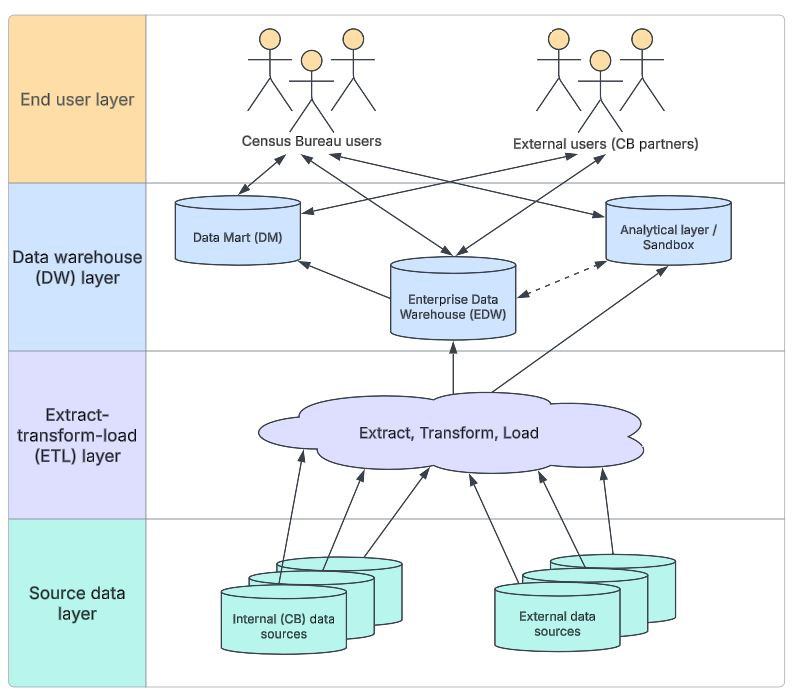
\includegraphics[width=1.0\textwidth]{Figures/Q1_BI_architecture.jpg}
  \caption{Proposed layered BI architecture for Census Bureaus.}
  \label{fig:BI_arch}
\end{figure}

As regards the ETL-layer, it is a compulsory part and component of any DW/BI-architecture, also in this case of Census Bureaus. Same with the data source layer, it is required in any constellation of a DW/BI-architecture. But what is particular in this case is that we believe Census Bureaus by default have several external data sources. And that most of these are tied to other authorities, either national (subject-specific) or regional (location-specific). But as or when data from the various internal and external data sources have been successfully loaded into the data warehouse, the main interest is in the DW layer and the end-user layer.  

To Census Bureaus our group recommends a DW layer having an enterprise data warehouse (EDW) as its foundation, but which is supplemented by a limited number of Data marts (DM). Here the EDW can be defined as a common storage of all historical data collected and gathered by a Census Burau. It means that the EDW represents the combined data model for a given Census Burau as a whole, and for all of its subject areas (Coursebook, 32.2). In in our BI-architecture the EDW provides all of the data to the data marts, whereas the data marts transfer no data to the EDW. These data marts could thus be categorized as dependent DM:s (Lecture 01 DW-[Ch31-6th Ed). The rationale for having an EDW as the main DW component is that it is the best alternative for gaining a consistent and all-encompassing view on the wide and diverse data held by a Census Bureau (Coursebook, 32.2). As Census Bureaus are central nodes for census data and other statistics in their respective nations, it is important that they as national authorities can act as the “single source of the truth”. Having an EDW implemented enables this. Another strength of the EDW is that it is more flexible than data marts (Lecture 02 DW-[Ch32-6th Ed]). This can be valuable for Census Bureaus e.g. if their data sources are volatile.  

The EDW that a given Census Bureau has should be accompanied by a limited number of separate data marts. The data marts should be allocated to the most important subject areas of that Census Bureaus. We think that the importance is partly dependent on the preferences of each Census Bureau, but generally those subject areas that are critical for society (healthcare, social insurance, energy) or that have large user groups (labour market, housing, construction) should be favoured. We think that the main advantage of implementing data marts for specific subject areas are that data can be supplied in forms that are tailored to the target user groups  (Coursebook, 31.4.1). However, keeping the number of data marts moderate is crucial, as to avoid creating a duplicate DW layer that would accelerate costs while impairing overall DW performance.   

One important component that must be part of the DW layer is the warehouse manager.  One of the main reasons for this is that warehouse managers are able to de-normalize data models and tables in the DW (Coursebook, 31.2.4). This feature is essential, as it enables analytical tools such as OLAP and data mining to access the EDW directly. However, in the figure describing our layered BI-architecture, we interpret the warehouse manager as an integrated part of the EDW.  

Analytic platforms, also known as sandboxes, are another component that adhere to the DW layer (Lecture 01 DW-[Ch31-6th Ed). These solutions are implemented and operate separate from the EDW, whereby they offer users own environments for storing unstructured data and experimenting with that to discover new patterns. Given the unstructured nature of the data and the experimental potentials in a sandbox, security becomes an important factor. As such, we recommend that only certain personnel employed at the given Census Bureau (power users) is given access to it.  The main usefulness of the sandbox is given by combining data sets from divergent subject areas, as to discover previously unknown associations or patterns. Another area of great use is to experiment with data before implementing it in the EDW to ensure compliance with the EDW and other factors. As such, the sandbox needs access to data beyond that of the EDW, which does not have as stringent, or necessarily any, demands on data transformation. In order to not overly complicate our architecture figure, we have however shown that it fetches data from the ETL layer like the EDW does. However, in practice the sandbox would have its own data fetch process. We recommend that Census Bureaus implement either physical sandboxes or software-as-a-service (SaaS) sandboxes (Lecture 01 DW-[Ch31-6th Ed]). For more information about the usefulness of sandboxes for Census Bureaus, please see case question Q2.  

 

End user layers are in practice mandatory in BI-architectures of Census Bureaus. Without them users would be unable to analyse data in a DW, whereby the DW and all of its components would be more or less useless. The tools in the end user layer can be divided into four groups dependent on whether they are used for i) traditional queries and reports, ii) OLAP purposes, iii) data mining, or for iv) application development (Coursebook, 31.2.10). We argue that Census Bureaus need to invest in and take into active use tools belonging to the categories i-iii, as all three are necessary and as they complement each other. OLAP tools are needed for detailed and ad-hoc analyses of multidimensional data sets of larger sizes (Coursebook, 33.1). Data mining tools, in turn, are optimal to apply on extensive data sets, also called big data (Coursebook, 34.1).  A final thing that our group includes in the end user layer is a visualisation tool. Most often tools of this type are either integrated into OLAP tools (03 OLAP-[Ch33-6th Ed]). But if not, then a Census Bureau should install a separate visualization tool as to have it part of its BI-architecture. Data visualization has become increasingly popular as data grow in volume and complexity. Here the potential user groups include external users of Census Bureaus as well as citizens.  